%% for a german thesis use english,ngerman, the last is default.
%% for dutch use \def\Languages{english,dutch}
%% for English use \def\Languages{english},
%% or \def\Languages{english,british} if you prefer british as English style
\def\Languages{ngerman,dutch,english}
%----------------------------------------------------------
% DO NOT TOUCH THIS FILE UNLESS YOU KNOW WHAT YOU ARE DOING
%----------------------------------------------------------
\InputIfFileExists{infopage.txt}{%
  \def\InfoMissingWarning{}
}{%
  \def\InfoMissingWarning{
    
    {\centering \Large \bf The information in this page is not correct, please
      provide the information in the document infopage.txt in the root of this TeX project.}

    You can find an example infopage.text file name infopage.txt-example. One approach is copy and edit the copy.
  }
}

\providecommand\Languages{dutch,ngerman,english}
\documentclass[a4paper,11pt]{report}
% my own Itemize, Enumerate, and Description : a bit less spacy then the default
\newenvironment{Itemize} {
  \begin{itemize}{}%
    \setlength\topsep{0ex}%
    \setlength\parskip{0ex}%
    \setlength\partopsep{0em}%
    \setlength\parsep{0em}%
    \setlength\itemsep{0em}%
  }{\end{itemize}
}
\newenvironment{Enumerate}{
  \begin{enumerate}
    \setlength{\itemsep}{1pt}
    \setlength{\parskip}{0pt}
    \setlength{\parsep}{0pt}}
  {\end{enumerate}
}

\newenvironment{Description}{
  \begin{description}
    \setlength{\itemsep}{1pt}
    \setlength{\parskip}{0pt}
    \setlength{\parsep}{0pt}}
  {\end{description}
}

%% citation and bibliography style.
%% This style depends on 'sortname' and 'shorthand' fields in the bib file.
%% This gives you control on what is shown in the labels.
%% If you ommit the shorthand, the styles fall back to a numeric label

% load early
\usepackage[utf8]{inputenc}
\usepackage[T1]{fontenc}
%% biblatex options, defualt to numeric but also support
%% shorthand and sortname keys in bib file bibliography.
\usepackage[
backend=biber,
hyperref=true,
backref=true,
]{biblatex}
\DefineBibliographyStrings{english}{
  backrefpage={cited on p.},
  backrefpages={cited on pp.}
}
% end citation bibliography style.

% support multiple languages.
\usepackage[\Languages]{babel}
% define page layout
\usepackage[a4paper,includemp,pdftex,
      top=20mm,left=20mm,
      total={185mm,260mm},
      includeheadfoot,
      marginparwidth=30mm,
%      showframe
      ]{geometry}
      %%
\newcommand\Margin[1]{\marginpar{\sffamily\textbf{#1}}}
      
\usepackage{layout}
      
\usepackage{fancybox}
\usepackage[pdftex]{graphicx}
\usepackage{longtable}
\usepackage{times}
\usepackage{varioref}
% Use multiple references to the same footnote

\usepackage{amsmath}
\usepackage{textcomp}
\usepackage{wrapfig}
\usepackage{varioref}
\usepackage[dvipsnames]{xcolor}
\usepackage[avantgarde]{quotchap}
\usepackage{tikz}
% allow compact lists etc.
\usepackage{enumitem}
\usepackage{%
  array,
  booktabs,
  dcolumn,
  rotating,
  shortvrb,
  units,
  url,
  lastpage,
  longtable,
  lscape,
  multirow,
  amssymb,
  amsmath,
  float,
  chngpage,
  colortbl,
  times,
  csquotes,
}

\usepackage[yyyymmdd]{datetime}
\renewcommand{\dateseparator}{-}
\usepackage{listings}
\lstset{numbers=right} % to get out of the way with document line numbers
\definecolor{listinggray}{gray}{0.2}
\definecolor{lbcolor}{rgb}{0.95,0.98,0.98}

%% settings for listings and code snippets.
\lstset{
  backgroundcolor=\color{lbcolor},
  tabsize=4,
  %	rulecolor=,
  language=java,
  basicstyle=\scriptsize,
  upquote=true,
  aboveskip={1.5\baselineskip},
  columns=fixed,
  showstringspaces=false,
  extendedchars=true,
  breaklines=true,
  prebreak = \raisebox{0ex}[0ex][0ex]{\ensuremath{\hookleftarrow}},
  frame=single,
  showtabs=false,
  showspaces=false,
  showstringspaces=false,
  identifierstyle=\ttfamily\bfseries\color{Black},
  keywordstyle=\color{Violet}\bfseries,%[rgb]{0,0,1},
  commentstyle=\color{Sepia},
  xleftmargin=3.4pt, %% small margins
  xrightmargin=7.4pt, %% margin into marginparsep
  stringstyle=\color[rgb]{0.627,0.126,0.941}
}

%% to show bibtex entries in listintgs examples chapter.
\makeatother
\lstdefinelanguage{BibTeX}
{keywords={%
    @article,@book,@collectedbook,@conference,@electronic,@ieeetranbstctl,%
    @inbook,@incollectedbook,@incollection,@injournal,@inproceedings,%
    @manual,@mastersthesis,@misc,@patent,@periodical,@phdthesis,@preamble,%
    @proceedings,@standard,@string,@techreport,@unpublished%
  },
  comment=[l][\itshape]{@comment},
  sensitive=false,
}

\usepackage[final]{pdfpages}

\usepackage[pagewise,mathlines,displaymath]{lineno}
%\setpagewiselinenumbers
\modulolinenumbers[3]
\renewcommand{\linenumberfont}{\normalfont\tiny\color{gray}}
\usepackage{hyperref}
\hypersetup{
  colorlinks=true,
  colorlinks=true,
  linkcolor=BlueViolet,
  filecolor=DarkOrchid,
  citecolor=PineGreen,
  urlcolor=RoyalPurple,
}
\usepackage[toc,acronym,xindy]{glossaries-extra}
\usepackage{cleveref}[2012/02/15]
\crefformat{footnote}{#2\footnotemark[#1]#3}


\usepackage{lipsum}
\usepackage{metainfo}
\providecommand{\MineOnlyStart}{}
\providecommand{\MineOnlyEnd}{}

%----------------------------------------------------------
% DO NOT TOUCH THIS FILE UNLESS YOU KNOW WHAT YOU ARE DOING
%----------------------------------------------------------


% environment for a two column table with proper alignment
% usage
% \begin{infoblock}
% Property: & Info
% \end{infoblock}
\newenvironment{infoblock}{
\begin{table}[h!]
\begin{tabular}{@{}p{0.30\textwidth}>{\bfseries}l}
}{
\end{tabular}
\end{table}
}

% Simple command for a fancy that attracts attention.
% usage:
% \LongQuote{the text you are quoting}{the name of the author}
% Any name can be passed (e.g. \citet{author2000text})
\newcommand{\LongQuote}[2]{
\begin{flushright}
	\begin{minipage}{.9\linewidth}
	\textit{#1}
	\end{minipage}

	\textit{#2}
\end{flushright}
}


%\usepackage{natbib}
\usepackage[nottoc]{tocbibind}
\usepackage{titlesec}
\usepackage{fancyhdr}
\addtolength\headwidth\marginparwidth
\addtolength\headwidth\marginparsep
\setlength{\parindent}{0pt}
\setlength{\parskip}{.5\baselineskip}
\usepackage{adjustbox}
\usepackage[toc,page]{appendix}

% chapter titles theme.
\definecolor{gray75}{gray}{0.75}
\newcommand{\hsp}{\hspace{20pt}}
\titleformat{\chapter}[hang]{\Huge\bfseries}{\thechapter\hsp\textcolor{gray75}{|}\hsp}{0pt}{\Huge\bfseries}

% this alters "before" spacing (the second length argument) to 0
\titlespacing*{\chapter}{0pt}{0pt}{40pt}
\titlespacing{\chapter}{0pt}{-25mm}{40pt}

\fancypagestyle{fancy}{%
  \fancyhf{}
  \fancyfoot[C]{\thepage}
}

\fancypagestyle{chapter-header-style}{
  \fancyhead[LE,RO]{\thepage}
  \fancyhead[RE,LO]{\chaptername\ \thechapter\ --\ \leftmark}
  \fancyfoot{}
}

\fancypagestyle{appendix}{
  \fancyhf{}
  \fancyhead[LE,RO]{\thechapter-\thepage}
%  \fancyhead[RE,LO]{\chaptername\ \thechapter\ --\ \leftmark}
  \fancyfoot{}
}

\pagestyle{fancy}

\renewcommand{\chaptermark}[1]{%
  \markboth{#1}{}}

\addto\captionsdutch{%
  \renewcommand\appendixname{Bijlagen}
  \renewcommand\appendixpagename{Bijlage}
  \renewcommand{\refname}{Referenties}
  \renewcommand{\bibname}{Referenties}
}
\addto\captionsgerman{%
  \renewcommand\appendixname{Anhänge}
  \renewcommand\appendixpagename{Anhang}
  \renewcommand{\refname}{Verweise}
  \renewcommand{\bibname}{Verweise}
}
\providecommand\DefInfo[1]{ define \textbackslash{}#1 in file ``./infopage.txt''}
\providecommand\documentname{\DefInfo{documentname}}
\providecommand\studentname{\DefInfo{studentname}}
\providecommand\place{\DefInfo{place}}
\providecommand\snumber{\DefInfo{snummer}}
\providecommand\course{\DefInfo{course}}
\providecommand\period{\DefInfo{period}}
\providecommand\companyname{\DefInfo{CompanyName}}
\providecommand\companyaddress{\DefInfo{CompanyAddress}}
\providecommand\companypostcodecity{\DefInfo{companypostcodecity}}
\providecommand\companycountry{\DefInfo{companycountry}}
\providecommand\companycoach{\DefInfo{companycoach}}
\providecommand\companycoachmail{\DefInfo{companycoachmail}}
\providecommand\universitytutor{\DefInfo{universitytutor}}
\providecommand\universitytutormail{\DefInfo{universitytutormail}}
\providecommand\examiner{\DefInfo{examiner}}
\providecommand\externalexpert{\DefInfo{externalexpert}}
\providecommand\hasnda{\DefInfo{hasnda}}

% This macro '\define' puts the argument in em 
% and in boldface in the margin.
\providecommand{\define}[1]{% 1 argument
  \mbox{}{\textit{#1}}% italics or em
  \marginpar{\raggedright% no adjust
    \bfseries\hspace{0pt}#1}% bold
} % end of macro
\newcommand\Code[1]{\textbf{\texttt{#1}\ }}
\newcolumntype{g}[1]{%
    >{\raggedright\arraybackslash}%
    p{#1}%
}

\newcommand\itemcell[1]{%
  %\mbox{% uncomment for debug 
  \begin{minipage}[t]{\linewidth}%
      \begin{itemize}[leftmargin=3.5ex]%
        #1
      \end{itemize}%
  \end{minipage}\vspace{.4\baselineskip}%
  %}% uncomment
}


\newcommand\headcell[1]{%
  \begin{minipage}[c]{\linewidth}
    \vspace{.2\baselineskip}%
    \raggedright%
    \textbf{#1}
  \end{minipage}\vspace{.4\baselineskip}%
}

\newcommand\firstcell[1]{%
  \cellcolor{Gray}%
  \begin{minipage}[c]{\linewidth}%
    \vspace{.2\baselineskip}%
    \raggedright%
    \textbf{#1}
  \end{minipage}\vspace{.4\baselineskip}%
}

\newcommand\textcell[1]{%
  \fbox{%
    \begin{minipage}[t]{\linewidth}%
      \raggedright%
      #1
  \end{minipage}}\vspace{.4\baselineskip}%
}
\newlength{\BulletSize}
\setlength{\BulletSize}{1.5ex}
\definecolor{Gray}{gray}{0.9} % color used in table borders
\newlength{\TabColumnWidth} % for tables
\newcommand\CheckMarkGreen[1]{
\includegraphics[height=#1]{images/Check_Green_White.pdf}\hspace{2pt}}
\newcommand\CMark{\raisebox{-.1\BulletSize}{\CheckMarkGreen{\BulletSize}}}
\newcommand\CrossMarkRed[1]{
\includegraphics[height=#1]{images/Cross_red_circle.pdf}\hspace{2pt}}
\newcommand\XMark{\raisebox{-.1\BulletSize}{\CrossMarkRed{\BulletSize}}}
\newcommand\WarningMarkYellow[1]{
\includegraphics[height=#1]{images/Alert_Yellow_White.pdf}\hspace{2pt}}
\newcommand\WMark{\raisebox{-.1\BulletSize}{\WarningMarkYellow{\BulletSize}}}
\newcommand\FirstCell[1]{\cellcolor{Gray}\thead{#1}}
\newcommand\URLIcon[1]{
\includegraphics[height=#1]{images/URL.pdf}\hspace{2pt}}
\newcommand\UMark{\raisebox{-.1\BulletSize}{\URLIcon{\BulletSize}}}
\newcommand\itemC{\item[\CMark]}
\newcommand\itemX{\item[\XMark]}
\newcommand\itemW{\item[\WMark]}
\newcommand\itemU{\item[\UMark]}
\newcommand\MyURL[2]{\url{#1}{\UMark #1}}
\usepackage[avantgarde]{quotchap}
\renewcommand\chapterheadstartvskip{\vspace*{-5\baselineskip}}

\definecolor{codegray}{gray}{0.9}
\newcommand{\code}[1]{\colorbox{codegray}{\texttt{#1}}}
\InputIfFileExists{IncludeOnly.tex}{}{}

%\includeonly{chapters/chapter_1}
% provide data for title page
\IfFileExists{linenumberingOn}{\linenumbers}{}
\title{\documentname}
\author{\studentname}
\date{\place, \today}

% remember to provide data for information page in infopage.tex

\begin{document}
\IfFileExists{IncludeOnly.tex}{}{%
\maketitle

% Define roman numbering for the pages that do not belong to the main content
\pagenumbering{roman} 

% Include all the pre-chapters
\def\InformationPageTitle{Information Page}
\providecommand\InformationPageTitle{Information Page}
\InputIfFileExists{infopage.txt}{%
  \def\InfoMissingWarning{}
}{%
  \def\InfoMissingWarning{
    
    {\centering \Large \bf The information in this page is not correct, please
      provide the information in the document infopage.txt in the root of this TeX project.}

    You can find an example infopage.text file name infopage.txt-example. One approach is copy and edit the copy.
  }
}
\chapter*{\InformationPageTitle}
\InfoMissingWarning
%\section*{\InformationPageTitle}
%% provide default values


Fontys Hogeschool Techniek en Logistiek\\
Postbus 141, 5900 AC Venlo

\vspace*{1cm}
\noindent
{\centering \Large\bfseries
  \documentname

}

\vspace{1cm}

\begin{infoblock}
Name of student: & \studentname\\
Student number: & \snumber\\
Course: & \course\\
Period: & \period\\
\end{infoblock}

\begin{infoblock}
Company name: & \companyname\\
Address: & \companyaddress\\
Postcode, City: & \companypostcodecity\\
Country: & \companycountry\\
\end{infoblock}

\begin{infoblock}
Company coach: & \companycoach\\
Email: & \texttt{\href{mailto:\companycoachmail}{\companycoachmail}}\\
University coach: & \universitytutor\\
Email: & \texttt{\href{mailto:\universitytutormail}{\universitytutormail}}\\
\end{infoblock}

\ifx\examiner\empty
\relax
\else
\ifx\externalexpert\empty
\relax
\else
\begin{infoblock}
  Examinator: & \examiner\\
  External domain expert: & \externalexpert\\
\end{infoblock}
\fi
\fi


\begin{infoblock}
Non-disclosure agreement: & \hasnda
\end{infoblock}
\clearpage
\chapter*{Preface}

Thanks to all the students that showed me there is always room for improvement.

In this 'thesis' I wrote down some of my annoyances in reading students work.

In several spots in this thesis I write 'I' or 'we', which is bad style in a normal thesis.
However, because I consider me, myself and my fellow teachers main stakeholders in all of your writing, I allow myself to do that here. \textit{Do not do that at home} (for your own thesis that is).

Pieter van den Hombergh,\\
Venlo 2024-04-26

\chapter*{Summary}
% No generated number
% add name to toc
I will not bore you with a summary. That would spoil the fun.

\textit{Summaries are overrated.}

\section*{TLDR;}

If that is not short enough:
\begin{Description}
\item[For the wordies] If you prefer word or some other ``word processor'', read
the improvement suggestions in \vref{sec:pdffromuml} and \vref{sec:stylish}.
\item [For all] Things to avoid when including code see \vref{chap:listings} and forget the rest. That to the wordies too.
\end{Description}



\chapter*{Samenvatting/Zusammenfassung}
TODO

\addcontentsline{toc}{chapter}{Statement of Authenticity}
\section*{Statement of Authenticity}
\sloppypar
I, the undersigned, hereby certify that I have compiled and written the attached document / piece of work and the underlying work without assistance from anyone except the specifically assigned academic supervisors and examiners. This work is solely my own, and I am solely responsible for the content, organization, and making of this document / piece of work.

I hereby acknowledge that I have read the instructions for preparation and submission of documents / pieces of work provided by my course / my academic institution, and I understand that this document / piece of work will not be accepted for evaluation or for the award of academic credits if it is determined that it has not been prepared in compliance with those instructions and this statement of authenticity.

I further certify that I did not commit plagiarism, did neither take over nor paraphrase (digital or printed, translated or original) material (e.g. ideas, data, pieces of text, figures, diagrams, tables, recordings, videos, code, ...) produced by others without correct and complete citation and correct and complete reference of the source(s). I understand that this document / piece of work and the underlying work will not be accepted for evaluation or for the award of academic credits if it is determined that it embodies plagiarism.

\vspace*{1cm}

\begin{infoblock}
  Name: & \studentname \\
  Student Number: & \snumber \\
  Place/Date: & \place, \today
\end{infoblock}

Signature:  \\
\IfFileExists{authenticity_signature.png}{%
  \hspace{2cm}%
  \includegraphics[width=.4\linewidth]{authenticity_signature.png}%
}{\fbox{\begin{minipage}{.6\linewidth}\sloppypar
      If you add a file called \texttt{authenticity\_signature.png} to root
      folder of your build, that will be included as signature here, instead of this text block.
    \end{minipage}
  }}

\clearpage
%% usual tables like table of contents, table of figures etc.
\IfFileExists{IncludeOnly.tex}{}{
\tableofcontents
\clearpage
\listoffigures
\clearpage
\listoftables
\clearpage
}
}

% Define arabic numbering for the pages that belong to the main content
\pagenumbering{arabic} 

% Define page heading style
\pagestyle{chapter-header-style}

% Include chapters
\chapter{Give me a meaningfull Title}
This is a bachelor thesis template you can use without any configuration or weird internal dependencies. Compiles from the get-go.

Here is an example reference of a website. \citep{google}

Here is an example reference of a book. \citep{goetz2006java}

Here is an example reference of an article. \cite{cattell2011scalable}

\chapter{Lipsum}
Demo text

but of course: TODO

\lipsum[2-4]

\chapter{More to read}
TODO
\chapter{Design}
TODO
\chapter{Implementation}
TODO

\begin{figure}
  \begin{minipage}{.9\linewidth}
    \textbf{DEMO}
  \lipsum[5]
  \end{minipage}
  \caption{\label{fig:minipagedemo} Minipage inside a figure}
\end{figure}

\chapter{Conclusion}
TODO
\chapter{Recommendations}
TODO
\chapter{Tips and Tricks}

\begin{itemize}
\item Either install Latex on your own machine, maybe in a docker-image, or use overleaf. \\
    On your own machine, the compilation will commence more quickly. There is also no compilation timeout, which you may run into with overleaf.
\item actively use $\backslash$include (for chapters) and $\backslash$input to break you 
 big document into smaller parts. If you then have a file called IncludeOnly.tex in your root dir, only the chapters in that file will be included. In this way it is easy to make something for your reviewers, but also speeds up the compilation process drastically, which is nice while you are editing and you work (re)view-driven.
\item If you add pictures or tables, always choose vector format. Never jpeg unless it is a photo, png only for screenshots, which you should try to avoid. In the drawing tool (Visual Paradigm, Umlet, drawio)  you can most likely export in pdf format which you can include with $\backslash$includegraphics. If you have svg, which the other popular vector format, you can use a conversion tool to turn it into a pdf. Inkscape, which is available on all relevant platforms, does the trick for me.
For tables, a spreadsheet(excel libreoffice calc) is a reasonable choice. Export the selection as pdf with no borders. May use a tool to clip/crop off the white borders. pdfcrop works for me there.
\end{itemize}

\begin{figure}[htbp]
\caption{Example svg image}
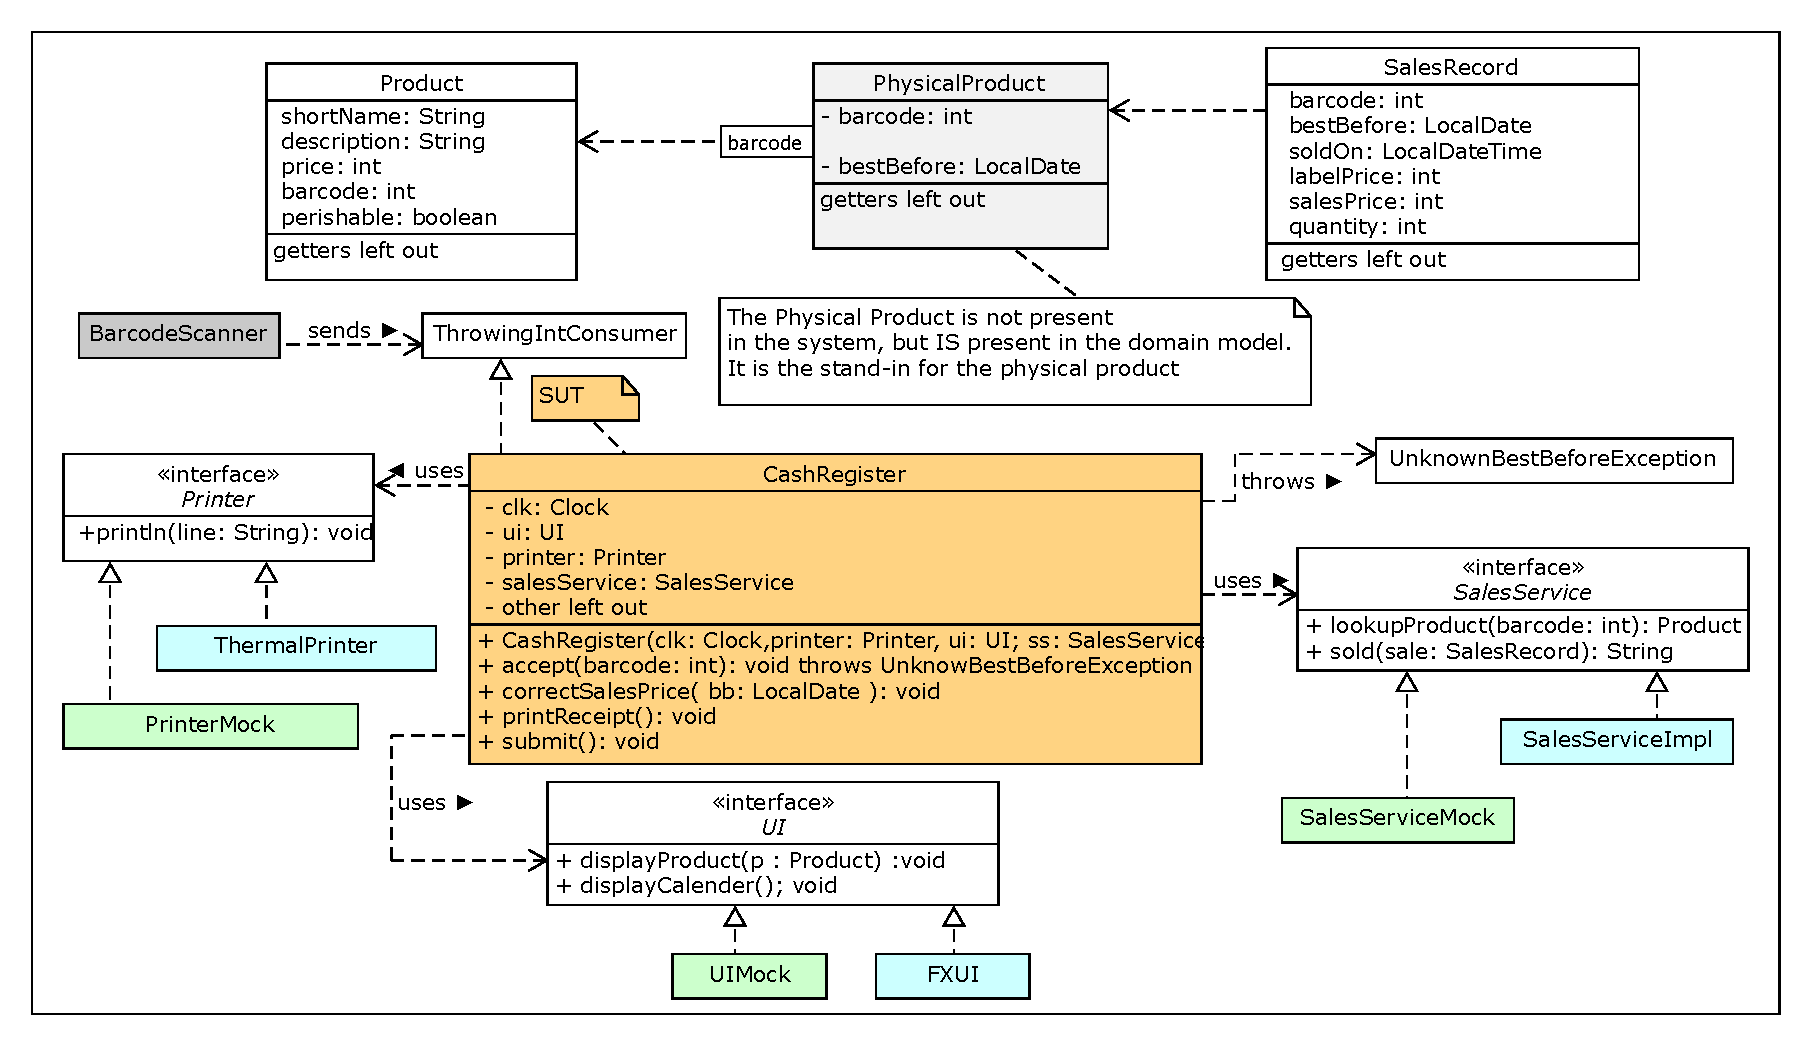
\includegraphics[width=\linewidth]{images/perishablesales.pdf}
\end{figure}

Try to select text in the image and zoom in and the advantages become apparent.
\chapter*{Self Reflection}

Here you can write your self reflection. You can use the table below to indicate the learning goals/competences.

\begin{table}[H]
	\centering
	\begin{adjustbox}{width={\textwidth}}
		\small
	\begin{tabular}{|c|c|c|c|c|c|c|c|}
		\hline
		& Manage & Analyse & Advice & Design & Implement & Professional Behaviour & Research Skills \\ \hline
		User-Interface & & &  & & & & \\ \hline
		Business Processes & &  &  & & & & \\ \hline
		Infrastructure & &  & &  & & & \\ \hline
		Software &  &  &  &  &  & & \\ \hline
		Hardware Interfacing & & & & & & & \\ \hline
		Professional Skills & & & & & &  &  \\ \hline
	\end{tabular}
\end{adjustbox}
	\caption{Project Skills Level}
	\label{currentskills}
\end{table}

%% supress post file when not required
\IfFileExists{IncludeOnly.tex}{}{%

% Set bibliography style to Harvard
\bibliographystyle{abbrvnat}

% Add the bibliography at the end
\bibliography{references}

% Add appendix
\begin{appendices}
	\begin{appendices}
\thispagestyle{empty}
    \renewcommand*{\thepage}{\thechapter-\arabic{page}}%
%% use appendix id + and number as page number.
\pretocmd{\chapter}{%
    \clearpage%
    \renewcommand*{\thepage}{\thechapter-\arabic{page}}%
  }{}{}
  % reset page numbers for appendix
  \pagenumbering{arabic}
  \chapter{Some macro examples}

The first macro defines a new environment.
An environment is something with $\backslash$begin\{environmentname\} and $\backslash$end\{environmentname\}, like an itemize list.
I wanted to tweak the standard lengths that are used, because I found the defaults a bit too spacy.

\begin{lstlisting}[caption={Tighter itemize}]
\newenvironment{Itemize} {
  \begin{itemize}{}% start of envionment with all the settings
    \setlength\topsep{0ex}%
    \setlength\parskip{0ex}%
    \setlength\partopsep{0em}%
    \setlength\parsep{0em}%
    \setlength\itemsep{0em}%
  }{\end{itemize}% end of the environmet
}
\end{lstlisting}


  \pagenumbering{arabic}
  \chapter{Include Listings}

The listing in \vref{lst:proper} was included with this code

\begin{lstlisting}
\lstset{%first some settings
  numbers=right, % number the lines
  numberstyle={\tiny\color{gray}},frameround=tttt,framerule=1pt,rulesepcolor=\color{gray},
  framexrightmargin=5mm
}
\end{lstlisting}

followed by

\begin{lstlisting}
  \lstinputlisting[language=java, firstline=1,firstnumber=1,
  lastline=39,numbers=right,basicstyle={\tiny\ttfamily},
  caption={The proper way to show your code.}
  ]{code/DAO.java}
\end{lstlisting}
      
  \pagenumbering{arabic}
  \chapter{Include using pdfpages}
Include the whole pdf with all pages and some scale down to have our own page numbering.
The pdf has been created from a website using the ``print to pdf'' feature of the \textbf{firefox} web browser which by the way has a very nice pdf viewer with annotation features.
\lstset{language=[LaTeX]TeX}
\begin{lstlisting}[caption={code to include next pages as pdf}]
 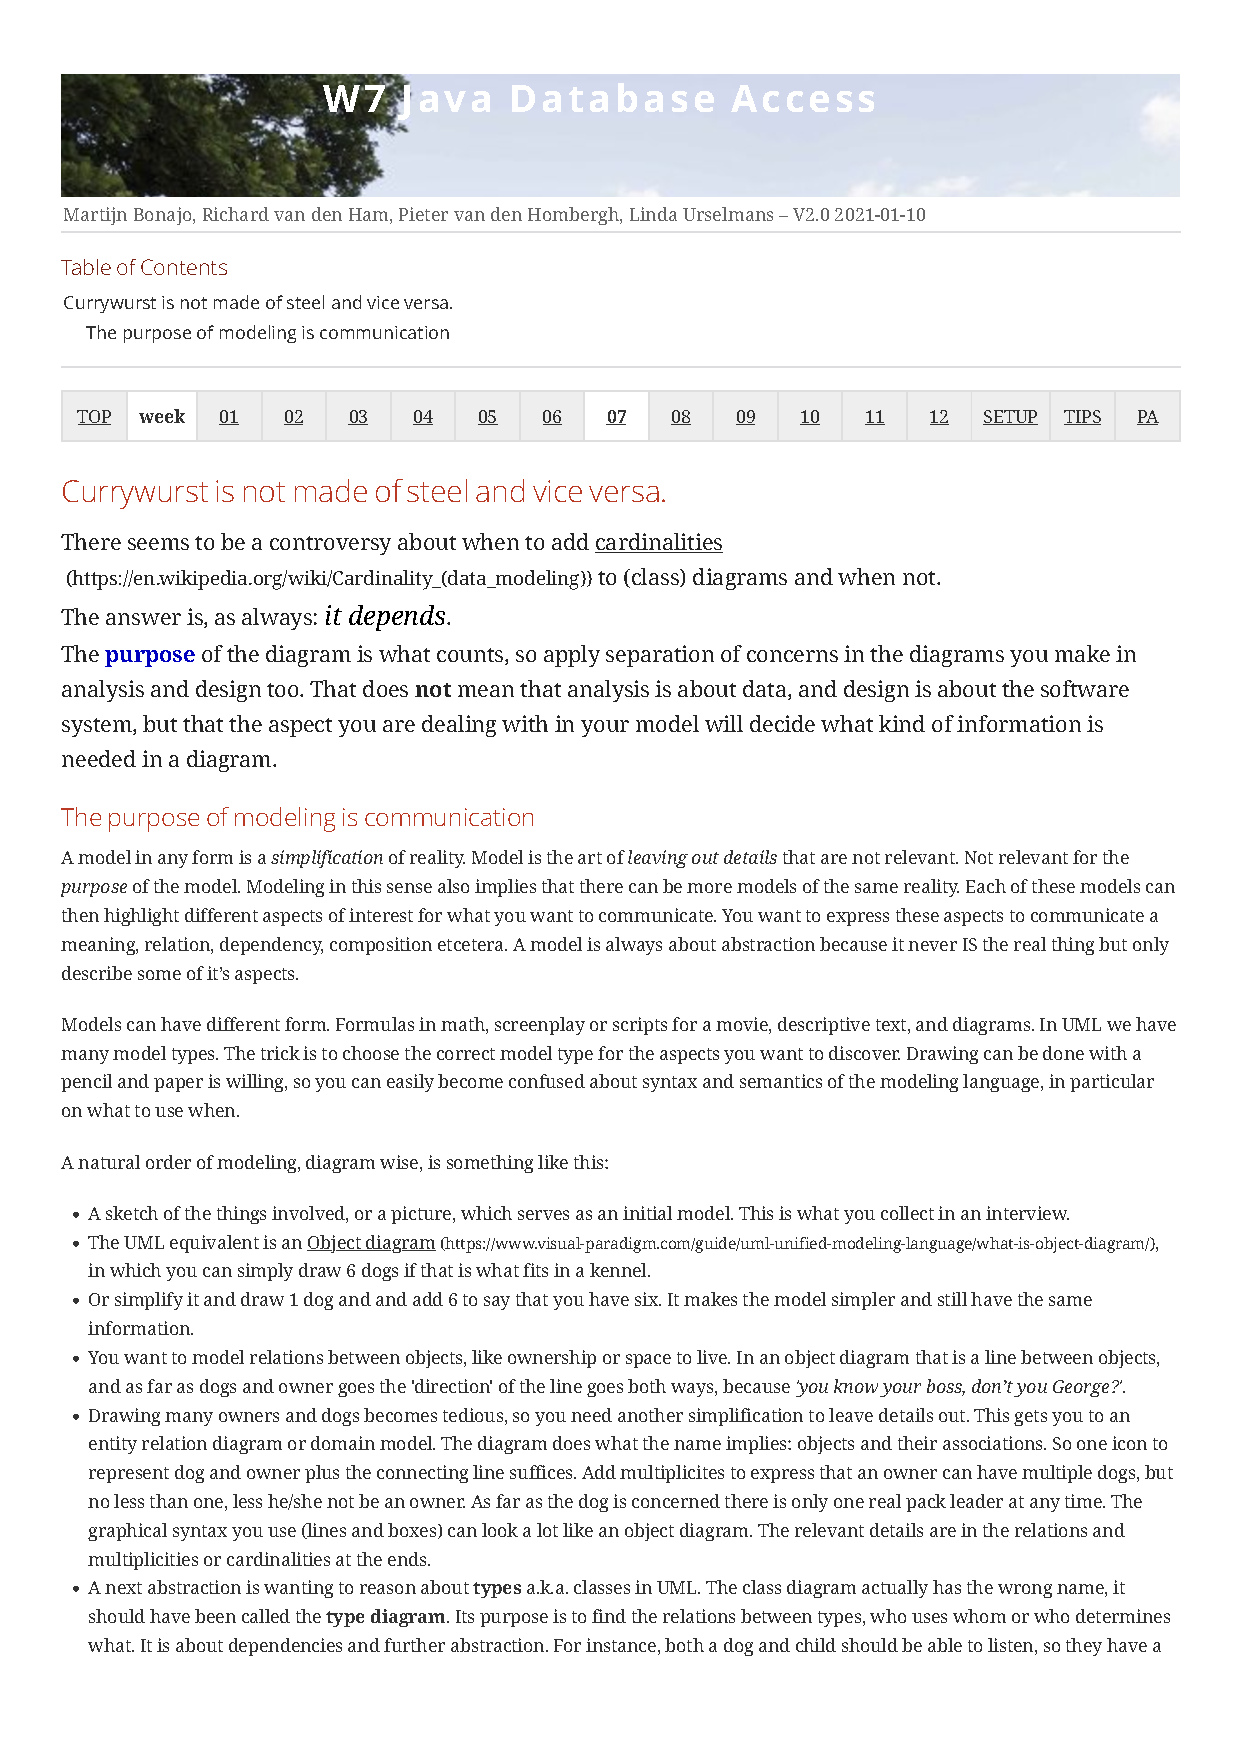
\includepdf[scale=0.9,pages=-,pagecommand={\pagestyle{fancy}}]{appendix/sausageisnotsteel.pdf}
\end{lstlisting}

If you make the documents intended for the appendix in \LaTeX\ too, you should of course simply $\backslash$include them in your report, as all but the last appendix here have been done.
% \pagestyle{empty}
%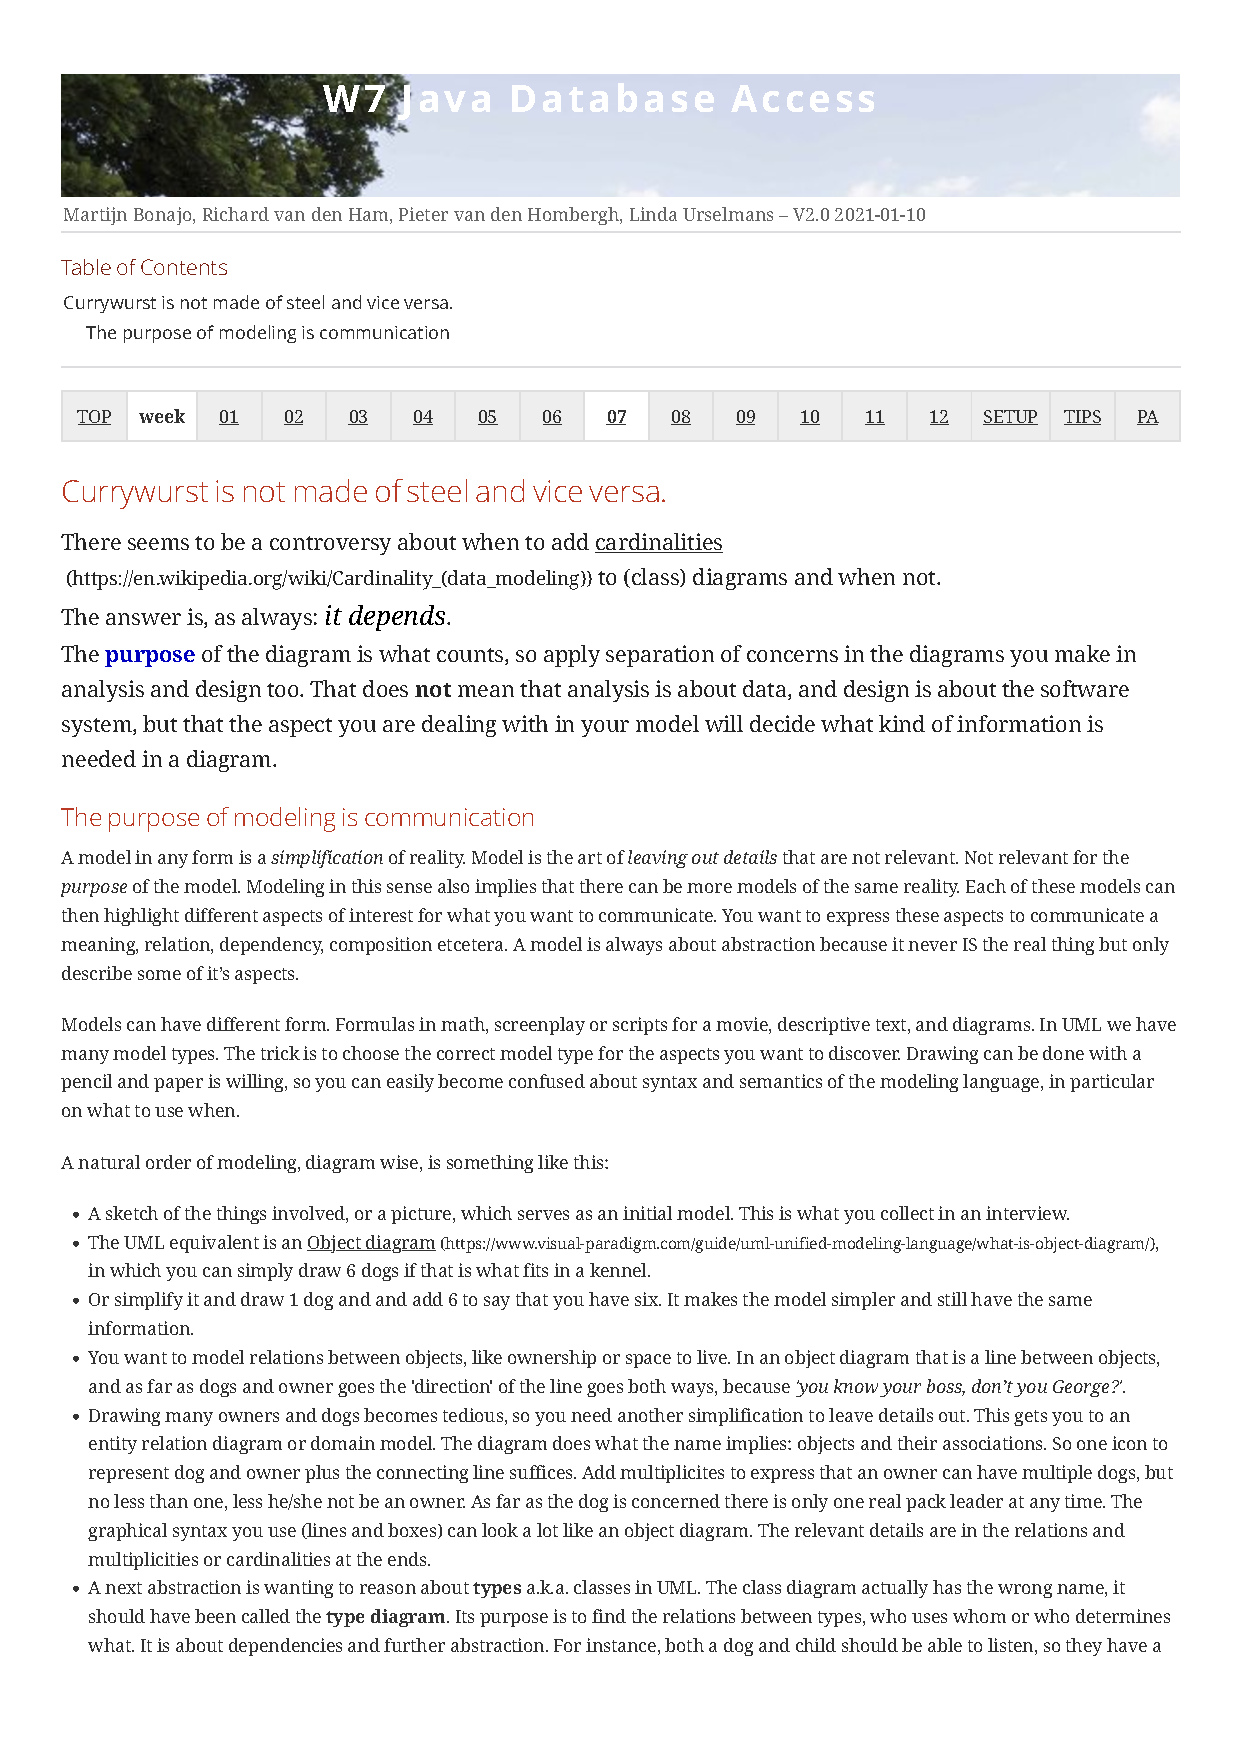
\includepdf[scale=0.9,pages=-,pagecommand={\pagestyle{fancy}}]{appendix/sausageisnotsteel.pdf}
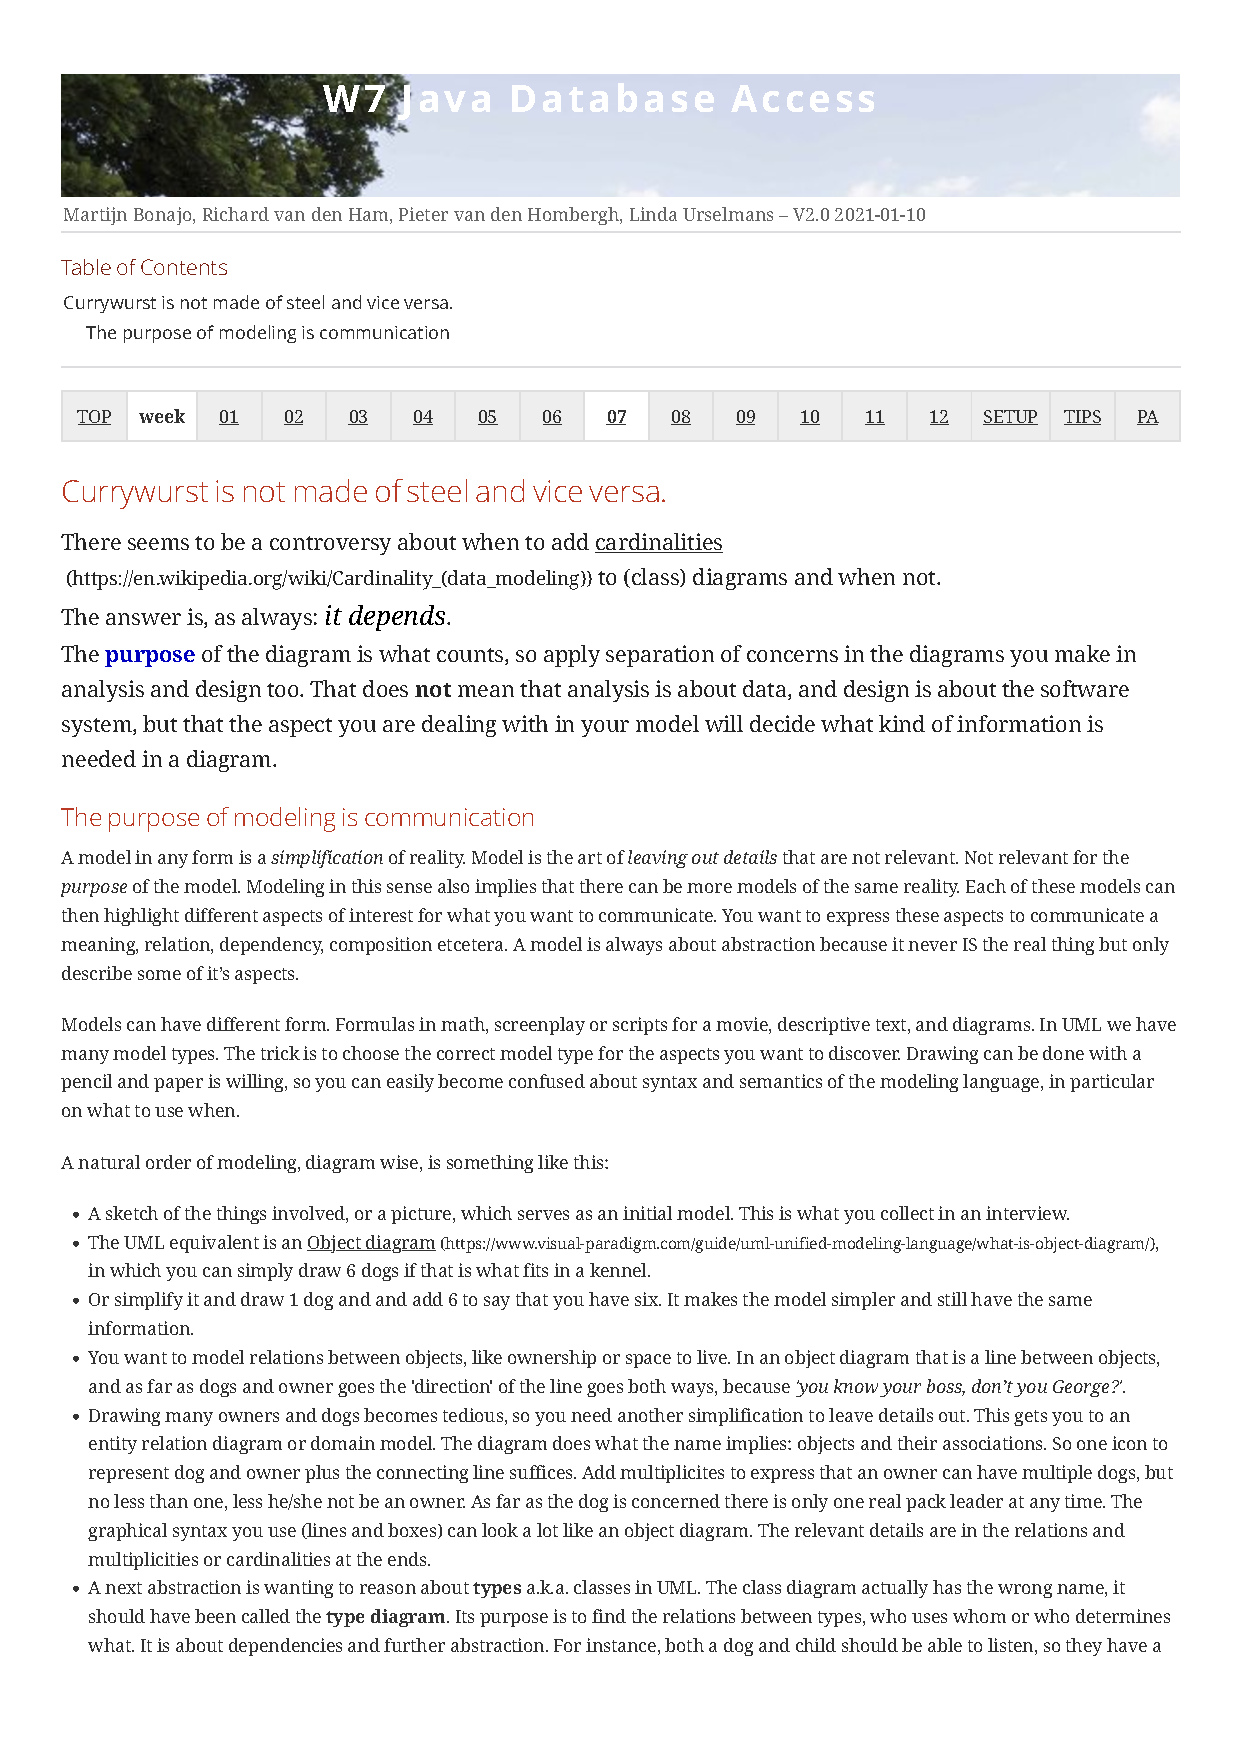
\includepdf[scale=0.9,pages=-,pagecommand={\thispagestyle{appendix}}]{appendix/sausageisnotsteel.pdf}


  \pagenumbering{arabic}
  \chapter{Counting words}

It is mandatory to include the word count of your thesis in the
information page. There are many constructs shown on the Internet but
we choose to go for the simplest solution possible.

\section{What to count}
It is resonable to only count the words in the report proper.
This implies only counting the words in the chapters, which is easy
enough by using the \texttt{texcount} command with a \define{\gls{glob}} for the
chapters: \texttt{chapters/*.tex}

\section{How to count}
\begin{lstlisting}[language=sh]
texcount  -inc -sum  -1 chapters/*.tex > wordcount.txt
\end{lstlisting}

\section{When to count}
To make sure that the word count in the file is updated in the
whenever a chapter file changes, we use the Makefile.

In the Makefile we make the \texttt{wordcount.txt} file dependent on the
chapter files with this simple rule:

\begin{lstlisting}[language=make,showtabs]
wordcount.txt: chapters/*.tex
	texcount  -inc -sum  -1 chapters/*.tex > wordcount.txt
\end{lstlisting}

and make the main.pdf file dependent on the \texttt{wordcount.txt} file as
well.

When that does not work for you, maybe, because you cannot or will not
use \texttt{make} in your environment, then execute the
\texttt{texcount} as given above in the terminal.

Even simpler, delete the \texttt{wordcount.txt} file and run pdflatex
again.


\end{appendices}

\end{appendices}
}
\end{document}
